% =============================================================================
%  Romanization Flattens the Field
%  ACL submission, anonymous review version.
%
%  COMPILER: XeLaTeX (required, for the Sinhala examples).
%  In Overleaf: Menu -> Compiler -> XeLaTeX.
%
%  Switch \usepackage[review]{acl} to \usepackage{acl} for camera-ready, or to
%  \usepackage[preprint]{acl} for a non-anonymous preprint with page numbers.
% =============================================================================
\documentclass[11pt]{article}
\usepackage[review]{acl}

\usepackage{microtype}
\usepackage{graphicx}
\usepackage{booktabs}
\usepackage{amsmath}
\usepackage{amssymb}
\usepackage{multirow}
\usepackage{array}
\usepackage[normalem]{ulem}

% ---- fonts -------------------------------------------------------------------
% XeLaTeX font setup. TeX Gyre Termes is metric-compatible with Times.
\usepackage{fontspec}
\setmainfont{TeX Gyre Termes}
\setsansfont{TeX Gyre Heros}
\setmonofont{TeX Gyre Cursor}[Scale=MatchLowercase]

% Sinhala. If Overleaf cannot find this face, substitute "Noto Sans Sinhala".
\newfontfamily\sinhalafont{Noto Serif Sinhala}[Script=Sinhala, Scale=MatchLowercase]
\newcommand{\si}[1]{{\sinhalafont #1}}

% ---- helpers -----------------------------------------------------------------
\newcommand{\rom}[1]{\textit{#1}}                 % Romanized Sinhala
\newcommand{\bpb}{\textsc{bpb}}
\newcommand{\bpw}{\textsc{bpw}}
\newcommand{\bpc}{\textsc{bpc}}
\newcommand{\mcc}{\textsc{mcc}}
\newcommand{\ssig}[1]{#1}
\newcommand{\nsig}[1]{#1}
\newcommand{\pkg}{\texttt{sinlipi}}

% LaTeX's \input confuses the alignment scanner inside a tabular, so the
% machine-generated table bodies are pulled in with the TeX primitive instead.
\makeatletter
\newcommand{\rows}[1]{\@@input #1 }
\makeatother

% Anonymous placeholders. Replace both before camera-ready.
\newcommand{\anonrepo}{\url{https://anonymous.4open.science/r/sinhala-script-robustness}}
\newcommand{\pkgurl}{\url{https://pypi.org/project/sinlipi}}

\title{Romanization Flattens the Field: Tokenizer-Independent and Downstream\\
Evidence of Script Fragility in Sinhala}

\author{Anonymous ACL submission}

\begin{document}
\maketitle

\begin{abstract}
Sinhala is written two ways online. Formal text uses the native script, while
everyday messaging is dominated by Romanized Sinhala typed in Latin letters. A
recent benchmark reported that language models are roughly 300 times worse at
Romanized than at native Sinhala, and that model scale predicts nothing. We show
that both conclusions are shaped by the metric. Re-measuring 31 checkpoints with
tokenizer-independent bits per byte, the ranking induced by perplexity turns out
to be uncorrelated with the ranking induced by bits per byte
($\rho = 0.08$), because perplexity mostly tracks how finely a tokenizer shreds
Sinhala. The 300-fold gap becomes 2.14 bits per byte, and scale does predict
native-script ability once the confound is removed. We then run the first
downstream evaluation of Sinhala script variation, covering three tasks, 9{,}479
items and ten instruction-tuned checkpoints under both scripts. Romanization
compresses a 22.4 point spread in native-script accuracy into 6.7 points, and the
loss a model suffers is almost exactly proportional to how much native-script
ability it had to begin with ($R^2 = 0.97$). On offensive-language detection,
accuracy barely moves while Matthews correlation loses 60\% of its value. The
effect is not a tokenization-length artifact: Romanized prompts are shorter in
tokens for every model we test. Finally, absolute bits per byte predicts
downstream script fragility, whereas the bits-per-byte \emph{gap} predicts
nothing.
\end{abstract}

% =============================================================================
\section{Introduction}
\label{sec:intro}

Sinhala is an Indo-Aryan language with about 17 million speakers and a script of
its own \citep{ranasinghe-etal-2025-sold}. Like several South Asian languages, it
has an everyday orthographic split. Formal and published writing uses the native
Sinhala script, but comments, chat and social media are dominated by Romanized
Sinhala, informally called Singlish, in which the same language is typed with
Latin letters. The Romanized form has no standard spelling, so
\si{කොහොමද} (``how are you'') is typed \rom{kohomada}, \rom{kohomd} or
\rom{kohomade} depending on the writer.

This is not a marginal input condition. In a comparable setting for Indian
languages, \citet{khullar-etal-2025-scriptgap} found that 83\% of Hindi and 73\%
of Telugu messages sent to a real maternal-health service were Romanized, and
that models handled those messages measurably worse. Anyone deploying a Sinhala
system for content moderation or user support is therefore serving mostly
Romanized input while evaluating on native-script benchmarks.

\citet{rajapakse-weerasinghe-2026-script} gave the first systematic measurement
for Sinhala. Benchmarking 24 open-weight models with perplexity, they reported a
median 312-fold degradation from native to Romanized text and no correlation
between parameter count and script handling. Both findings are widely quotable,
and both rest on a metric that is not comparable across models. Perplexity is
normalised by token count, and token count for a given string depends entirely on
the tokenizer \citep{gao-etal-2020-pile, magnusson-etal-2024-paloma}. Sinhala is
exactly the setting where that matters, because tokenizers segment it very
differently \citep{petrov-etal-2023-tokenizers, ahia-etal-2023-languages}. The
same work also notes that perplexity says nothing about whether a model can still
do anything useful, and calls for downstream evaluation.

We take up both problems.

\paragraph{Fixing the metric changes the intrinsic picture.}
We recompute bits per byte, per character and per word for 31 checkpoints, 7 of
them new relative to prior work, over the same parallel corpus
(\S\ref{sec:intrinsic}). Our perplexities reproduce the published values, so the
differences that follow come from the metric and not the measurement. Across
checkpoints, perplexity and bits per byte are uncorrelated
($\rho = 0.08$, $p = 0.68$), and perplexity is instead almost fully explained by
tokenizer fertility ($\rho = -0.87$, $p < 10^{-9}$). The 300-fold gap corresponds
to 2.14 bits per byte, a factor of 4.4 per byte. Under bits per byte, scale
\emph{does} predict native-script ability ($\rho = -0.55$, $p = 0.001$), though
still not Romanized ability.

\paragraph{Romanization flattens rather than merely degrades.}
Native-script cost varies widely across checkpoints, from 16.3 to 34.1 bits per
word, while Romanized cost collapses into a 20.3 to 25.7 band. Twelve of the 31
checkpoints are actually \emph{cheaper} on Romanized text than on native text,
simply because they were bad at native Sinhala to start with. A held-out character
4-gram model fit on 400 sentences beats all 31 checkpoints on Romanized Sinhala.

\paragraph{The first downstream evidence for Sinhala.}
We evaluate ten instruction-tuned checkpoints on 9{,}479 items across
multiple-choice knowledge, offensive-language detection and physical commonsense,
under both scripts, for 189{,}580 generations (\S\ref{sec:extrinsic}). Every
comparison is paired and tested with McNemar's test under Holm correction. The
same flattening appears: a 22.4 point spread in native-script accuracy becomes
6.7 points. More precisely, the loss is proportional to how much a model had,
$\text{loss} = 0.78 \times \text{headroom above chance}$ with $R^2 = 0.97$, and
the same relation holds within the benchmark across 16 domain by difficulty cells.
We show the effect is not driven by token-length inflation or by output
degeneration.

\paragraph{A usable predictor, and a released transliterator.}
Absolute native-script bits per byte predicts the downstream gap
($\rho = -0.90$, $p = 0.0009$), while the bits-per-byte \emph{gap}, the quantity
prior work reports, predicts nothing ($\rho = -0.07$, $p = 0.86$). Building the
Romanized side required a native-to-Latin transliterator, the opposite of the
direction most Sinhala tools support. Ours beats three alternatives on all three
reference corpora, 755{,}000 human-romanized items, and we release it as a
pip-installable package.

% =============================================================================
\section{Related Work}
\label{sec:related}

\paragraph{Sinhala and low-resource evaluation.}
Sinhala is classified as low-resource and its tooling has grown in a fragmented way
\citep{desilva-2019-survey, ranathunga-de-silva-2022-languages,
joshi-etal-2020-state}. Recent resources are almost entirely native-script:
SinhalaMMLU \citep{pramodya-etal-2025-sinhalammlu}, SOLD
\citep{ranasinghe-etal-2025-sold}, the Sinhala split of Global PIQA
\citep{desilva-ranathunga-2026-sinhalapiqa, chang-etal-2025-globalpiqa} and encoder
work such as \citet{dhananjaya-etal-2022-bertifying}. The only benchmark treating
script as a variable is \citet{rajapakse-weerasinghe-2026-script}, which we extend.

% TODO before camera-ready: \citet{chamikara-sumanathilaka-2026} (ICARC 2026,
% Romanized Sinhala hate speech with multilingual encoders) is the closest
% same-language, same-task prior work and belongs in the paragraph below. We could
% not reach the IEEE record to verify its metadata, so it is left uncited. Confirm
% the entry in custom.bib and then add, e.g.: "The closest same-language work is
% \citet{chamikara-sumanathilaka-2026}, who fine-tune multilingual encoders on
% transliterated SOLD; we instead measure general-purpose models zero-shot."
\paragraph{Romanization gaps elsewhere.}
Romanized South Asian text has been studied mainly as a resource and identification
problem \citep{roark-etal-2020-dakshina, benton-etal-2025-improving}.
\citet{j-etal-2024-romansetu} show romanization can \emph{help} when models are
adapted for it, the mirror image of our zero-shot setting. Closest in spirit is
\citet{khullar-etal-2025-scriptgap}, who find F1 drops up to 24 points on Romanized
clinical queries. We add a paired item-level design with a competence screen, a
tokenizer-independent intrinsic account of the same models, and a test of whether
the gap is a tokenization artifact.

\paragraph{Why not perplexity.}
Bits per byte exists so that models with different vocabularies can be compared
\citep{gao-etal-2020-pile}, and Paloma adopts it for that reason
\citep{magnusson-etal-2024-paloma}. Tokenizers are known to treat languages very
unequally \citep{petrov-etal-2023-tokenizers, ahia-etal-2023-languages}. To our
knowledge ours is the first work to show that, for a specific language, the
substantive conclusions of a published benchmark reverse when the normaliser
changes.

% =============================================================================
\section{Experimental Setup}
\label{sec:setup}

\subsection{Script conditions}

Every item is evaluated twice, once in the native script as published and once in a
Romanized form with identical content, so all comparisons are paired and differ only
in orthography. This avoids the confound of using an independently authored
Latin-script Sinhala set, of which Global PIQA does publish one.

\subsection{Data}

Table~\ref{tab:datasets} lists the evaluation sets. The intrinsic corpus is the
parallel set released with \citet{rajapakse-weerasinghe-2026-script}: 500
sentence pairs in which the Romanized side was typed by native speakers rather
than generated. This matters, because it means the intrinsic results carry no
dependence on our own transliterator. A separate 500-sentence corpus of authentic
mixed-script text supports a secondary condition.

For the downstream tasks we use every available item with no sampling. SinhalaMMLU is a
6{,}879-item, curriculum-aligned multiple-choice benchmark in the style of MMLU
\citep{hendrycks-etal-2021-mmlu}, over six domains and three difficulty levels; 2{,}139 items have five options rather than four, so
random guessing scores 23.4\% rather than 25\%.\footnote{The public Hugging Face
release contains a 1{,}851-item sample. We obtained the full set from the
authors.} SOLD supplies the complete 2{,}500-item test split of a binary
offensive-language task where 40.6\% of posts are offensive, so always predicting
the majority class scores 59.4\%. Global PIQA, which follows PIQA
\citep{bisk-etal-2020-piqa}, contributes the 100 released Sinhala items, 77 of them
culturally specific.

\begin{table}[t]
\centering\small
\setlength{\tabcolsep}{3.4pt}
\begin{tabular}{@{}llrl@{}}
\toprule
\textbf{Set} & \textbf{Task} & \textbf{Items} & \textbf{Baseline} \\
\midrule
\multicolumn{4}{@{}l}{\emph{intrinsic}} \\
\quad Parallel   & LM cost, paired  & 500 & --- \\
\quad Mixed      & LM cost, single  & 500 & --- \\
\addlinespace[2pt]
\multicolumn{4}{@{}l}{\emph{downstream}} \\
\quad SinhalaMMLU & 4/5-way MCQ    & 6{,}879 & 23.4\% chance \\
\quad SOLD        & binary class.  & 2{,}500 & 59.4\% majority \\
\quad Global PIQA & 2-way MCQ      & 100     & 50.0\% chance \\
\bottomrule
\end{tabular}
\caption{Evaluation data. Every downstream item is scored under both script
conditions, giving 18{,}958 prompts per checkpoint.}
\label{tab:datasets}
\end{table}

\subsection{Building the Romanized side}
\label{sec:translit}

Almost every Sinhala transliteration tool runs Latin to native
\citep{de-mel-etal-2025-sinhala, sumanathilaka-etal-2025-swabhasha}. We need the
reverse. We implemented a deterministic grapheme-level transliterator that parses
Sinhala as the abugida it is, walking the string and emitting a consonant's Latin
form followed by either an explicit vowel sign, nothing when the virama
\si{්} (U+0DCA) cancels the inherent vowel, or the inherent \rom{a} otherwise. It uses the
digraph conventions Sinhala speakers actually type, so \si{ත} is \rom{th} and
\si{ව} is \rom{w} rather than \rom{v}. It runs locally with no model or network,
covers every input, and is reversible only up to the consonant merges that casual
Singlish also collapses, such as \si{ට}/\si{ත} both becoming \rom{t}/\rom{th}.
For example \si{වෙසක් උත්සවයේදී බෞද්ධයින්} becomes
\rom{wesak uthsawayeedii bauddhayin}, and \si{ප්‍රතිපත්ති}, whose conjunct is
joined by a zero-width joiner, becomes \rom{prathipaththi}.

We validated it against 755{,}000 human-romanized items from the Swa-bhasha
Resource Hub \citep{sumanathilaka-etal-2025-swabhasha}: 4{,}397 authentic
social-media sentence pairs, 450{,}587 words each carrying multiple accepted
spellings, and a fixed 300{,}000-sentence sample of a machine-augmented set used
only as a cross-check. Hypotheses are scored against the closest accepted
reference, case-folded, using character error rate, chrF
\citep{popovic-2015-chrf} and exact match. Table~\ref{tab:methods} compares our
method with Aksharamukha \citep{rajan-aksharamukha}, uroman
\citep{hermjakob-etal-2018-uroman} and the web romanizer released with
\citet{desilva-ranathunga-2026-sinhalapiqa}. Ours has the lowest character error
rate on all three corpora, and a paired Wilcoxon test separates it from every
alternative at $p < 10^{-90}$ on the two large corpora. The web tool is close once
its \rom{v} is rewritten to \rom{w}, which is a spelling convention rather than a
transliteration error, but it cannot romanize 17 sequences involving \si{ඤ} at
all and leaves Sinhala characters in 0.8\% to 2.5\% of its output.

The residual error is one systematic difference rather than phonemic mistakes. All
four methods double long vowels far more often than people do, 0.81 per word against
0.12, which is why we produce \rom{bas eka enna thawath welaawak\ yanawada?} where a
human wrote \rom{bus eka enna thawath welawak\ yanawada?}. Canonicalising that single
convention on both sides cuts character error rate to 0.040 on the word corpus. We
keep the uncanonicalised form, since over-regular spelling is conservative: it is
closer to a standard than real Singlish, so it should be easier for a model.

\begin{table}[t]
\centering\small
\setlength{\tabcolsep}{2.2pt}
\begin{tabular}{@{}lccccc c@{}}
\toprule
& \multicolumn{3}{c}{\textbf{CER} $\downarrow$} & \textbf{chrF} & \textbf{Exact} & \textbf{Cov.} \\
\cmidrule(lr){2-4}\cmidrule(lr){5-5}\cmidrule(lr){6-6}\cmidrule(lr){7-7}
\textbf{Method} & sent. & word & aug. & sent. & word & \% \\
\midrule
\rows{tables/tab_methods.tex}
\bottomrule
\end{tabular}
\caption{Transliteration quality against human references (4{,}397 sentence
pairs, 450{,}587 multi-reference words, 300{,}000 augmented sentences). Coverage
is the share of inputs the method produced any output for.}
\label{tab:methods}
\end{table}

\subsection{Models}

The intrinsic evaluation covers 31 decoder-only checkpoints from 350M to 14.7B
parameters, spanning the Llama \citep{grattafiori-etal-2024-llama3}, Qwen
\citep{yang-etal-2024-qwen2, yang-etal-2025-qwen3}, Gemma
\citep{gemmateam-2024-gemma2}, Mistral, BLOOM \citep{lescao-etal-2023-bloom}, OPT,
Pythia \citep{biderman-etal-2023-pythia} and Phi \citep{abdin-etal-2024-phi4}
families. Twenty-four match \citet{rajapakse-weerasinghe-2026-script}, and we add
three newer base checkpoints and four instruction-tuned counterparts. Appendix
Table~\ref{tab:modelids} gives every identifier.

The downstream evaluation needs models that follow a response format, so it uses
the ten instruction-tuned checkpoints in the pool, from 1.1B to 9B parameters.
Two of them turn out to be unable to follow the format at all in the native-script
condition, which we handle explicitly in \S\ref{sec:screen} rather than by
dropping them.

\subsection{Prompting and scoring}

All downstream prompts are zero-shot and greedily decoded with a 40-token limit. We
chose one template from three candidates using a pilot of 3{,}240 generations over
nine checkpoints, then applied it to every dataset and both script conditions. What a
paired comparison needs is not an optimal template but one that does not favour a
script, and in the pilot the winning template was the same under both scripts for all
three datasets. Answers are extracted by pattern match, and anything unparseable is
scored as wrong and reported separately as an invalid rate
(Appendix~\ref{sec:prompts}).

\subsection{Statistics}
\label{sec:stats}

Both conditions score the same items, so we use McNemar's exact or
continuity-corrected test \citep{mcnemar-1947, dror-etal-2018-hitchhikers} and
report the discordant pair counts. Within each dataset we control the family-wise
error rate over checkpoints with Holm's procedure \citep{holm-1979}. Confidence
intervals on gaps, macro-F1 differences and Matthews correlation differences come
from 10{,}000 paired item bootstrap resamples. For SOLD we lead with Matthews
correlation \citep{matthews-1975, chicco-jurman-2020} because the classes are
imbalanced and accuracy is close to the majority baseline. Item-level effects are
also fitted as logistic regressions with checkpoint fixed effects and
cluster-robust standard errors by item.

\subsection{The competence screen}
\label{sec:screen}

A model at chance in the native-script condition cannot lose anything by being
given Romanized input, so a small gap for such a model is evidence of nothing.
Reporting it alongside real effects would understate the phenomenon. We therefore
mark a checkpoint as \emph{competent} on a task when its native-script score is
above the guessing baseline at $p < 0.01$ under a Poisson-binomial null, and when
it does not put more than 90\% of its answers on a single option. Five of ten
checkpoints pass on SinhalaMMLU, five have a non-trivial native-script signal on
SOLD, and none pass on Global PIQA. All ten appear in every table.

% =============================================================================
\section{The Intrinsic Picture}
\label{sec:intrinsic}

\subsection{Metrics}

For a text $s$ we accumulate the model's total negative log-likelihood
$\mathrm{NLL}(s)$ in nats and divide by a unit of the text itself rather than by
its tokenization:
\begin{equation}
\bpb = \frac{\sum_s \mathrm{NLL}(s)}{\ln 2 \sum_s |s|_{\text{bytes}}},
\label{eq:bpb}
\end{equation}
and likewise per character (\bpc) and per whitespace word (\bpw). We pool numerator
and denominator over the corpus rather than averaging per-sentence ratios, so short
sentences do not dominate. Bytes are the standard choice
\citep{gao-etal-2020-pile}, but \bpw{} is sharpest for cross-script comparison,
because a sentence and its romanization contain the same number of words while
Sinhala UTF-8 spends 2.65 bytes per character against 1.00 for Latin.

As a sanity check, our recomputed perplexities reproduce the published values for
all 24 shared checkpoints, with median absolute deviation 0.05\% on native and
0.004\% on Romanized text. Everything below therefore reflects the metric, not a
different run.

\subsection{Perplexity ranks models by their tokenizers}

Figure~\ref{fig:ppl} makes the central methodological point. Across the 31
checkpoints, native-script perplexity and native-script bits per byte are
statistically unrelated ($\rho = 0.08$, $p = 0.68$; Romanized $\rho = 0.13$,
$p = 0.48$). Only one of the five best checkpoints by perplexity is also among the
five best by bits per byte. Gemma-2-9B ranks 26th of 31 on perplexity and 2nd on
bits per byte, and Qwen3.5-9B-Base moves from 28th to 6th.

The cause is visible in panel (b). Perplexity is almost fully explained by how
many tokens a tokenizer spends on a Sinhala word ($\rho = -0.87$, $p < 10^{-9}$),
which ranges from 4.3 for the Qwen3.5 and Gemma tokenizers to 14.2 for models
that fall back to bytes. Spreading the same loss over three times as many tokens
lowers per-token perplexity without the model knowing anything more. So a headline
perplexity comparison across model families on Sinhala is largely a comparison of
tokenizers, and reported perplexity ratios inherit the same problem.

Two conclusions follow. First, the reported 312-fold degradation is
mostly a tokenization effect. Our median ratio is 294-fold, but in bits per byte
the same gap is 2.14 bits, a factor of 4.4 per byte, and in bits per word it is
1.11 bits. Second, the finding that scale does not predict script handling does not
survive. Parameter count is uncorrelated with native perplexity ($\rho = 0.15$,
$p = 0.42$) but clearly correlated with native bits per byte ($\rho = -0.55$,
$p = 0.001$) and with mixed-script bits per byte ($\rho = -0.57$, $p = 0.0008$).
Scale does buy native-script ability. What it does not buy is Romanized ability,
where the correlation stays insignificant ($\rho = -0.28$, $p = 0.13$).

\begin{figure}[t]
\centering
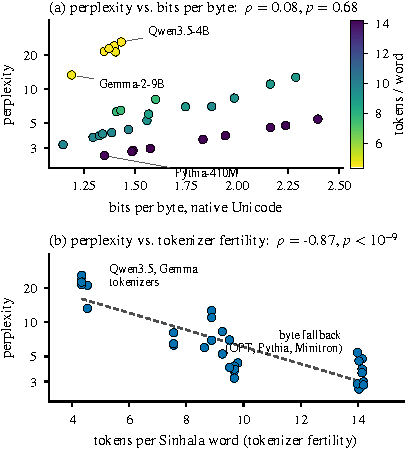
\includegraphics[width=\columnwidth]{figures/fig2_perplexity_artifact.pdf}
\caption{Perplexity does not measure what it appears to. (a) Across 31
checkpoints, native-script perplexity is unrelated to native-script bits per byte.
(b) It is instead almost fully determined by how many tokens the tokenizer spends
per Sinhala word.}
\label{fig:ppl}
\end{figure}

\subsection{Romanization flattens the field}

Figure~\ref{fig:flat}(a) shows the effect that motivates the rest of the paper.
Native-script cost spans 16.3 to 34.1 bits per word across checkpoints, a spread
of 17.7 bits. Romanized cost spans 20.3 to 25.7, a spread of 5.4. Regressing one
on the other, a full bit per word of native-script improvement buys only 0.14 bits
on Romanized text (95\% CI $[0.05, 0.25]$, $R^2 = 0.19$). Twelve of the 31
checkpoints are cheaper on Romanized than on native Sinhala, and which ones is
entirely predictable: the better a checkpoint is natively, the more it loses
($\rho = -0.88$ between native cost and the change, $p < 10^{-9}$). Romanized
Sinhala is a regime in which model quality has largely stopped mattering.

The mixed-script condition behaves quite differently and reproduces the earlier
finding. Native and mixed bits per byte are strongly rank-correlated
($\rho = 0.94$) with a median gap of only 0.49 bits, against $\rho = 0.41$ for
Romanized. Interleaving native tokens with Latin ones is a mild perturbation.
Replacing the script entirely is not.

\subsection{How much is that in absolute terms?}

Relative statements leave open whether models are merely worse or genuinely
uninformed. As a reference we fit add-$\alpha$ character $n$-gram models on the same
corpus under five-fold cross-validation, so each score is out of sample, and convert
to bits per byte. This is a cheap in-domain model and the comparison favours it in
that respect, but the size of the difference is still informative.
Table~\ref{tab:ngram} reports it, and Figure~\ref{fig:ngram} in the appendix plots
it. On Romanized Sinhala the best $n$-gram model reaches 2.64 bits per byte and
even a character bigram reaches 3.06, while the best of 31 checkpoints reaches 3.29
and the median 3.81. Not one checkpoint beats the bigram. On native Sinhala the
picture is ordinary, with the character trigram at 1.16 and one checkpoint below
it. Whatever these models know about Sinhala, they know it about the script rather
than the language.

\begin{table}[t]
\centering\small
\setlength{\tabcolsep}{4pt}
\begin{tabular}{@{}lcccc@{}}
\toprule
& \multicolumn{2}{c}{\textbf{Native Unicode}} & \multicolumn{2}{c}{\textbf{Romanized}} \\
\cmidrule(lr){2-3}\cmidrule(lr){4-5}
\textbf{Model} & \bpb{} & \#\,LMs $<$ & \bpb{} & \#\,LMs $<$ \\
\midrule
\rows{tables/tab_ngram.tex}
\bottomrule
\end{tabular}
\caption{Held-out character $n$-gram models against the 31 checkpoints.
``\#\,LMs $<$'' counts checkpoints that achieve lower bits per byte than the
$n$-gram model. No checkpoint beats a character bigram on Romanized Sinhala.}
\label{tab:ngram}
\end{table}

% =============================================================================
\section{Downstream Consequences}
\label{sec:extrinsic}

Table~\ref{tab:main} reports every checkpoint on every task.

\subsection{Multiple-choice knowledge}

Four of the five competent checkpoints lose significantly under Romanization after
Holm correction. Qwen3.5-9B falls from 44.1\% to 28.7\%, a 15.5 point drop
(95\% CI $[14.0, 16.9]$, 1{,}892 against 828 discordant pairs), Qwen3.5-4B loses
10.6 points, Llama-3.1-8B-Instruct 5.4 and Qwen2-7B-Instruct 2.0. The fifth,
Hormoz-8B, starts only 2.5 points above chance and loses 0.8 points, which is not
significant. Pooled over the cohort the gap is 6.9 points
(95\% CI $[6.3, 7.5]$, $n = 34{,}395$ paired items), and a logistic fit with
checkpoint fixed effects and item-clustered errors puts the odds ratio for
Romanized input at 0.68 ($p < 10^{-30}$).

Read as levels the result is starker. Figure~\ref{fig:flat}(b) shows native-script
accuracy spanning 22.4 points while Romanized accuracy spans 6.7. Romanized accuracy
never exceeds 28.7\% against a 23.4\% chance baseline, so the best checkpoint keeps
5.2 of its 20.7 points of headroom, and regressing Romanized on native accuracy gives
a slope of 0.22 (95\% CI $[0.12, 0.54]$). The six checkpoints showing no gap are the
six already at chance.

\begin{figure*}[t]
\centering
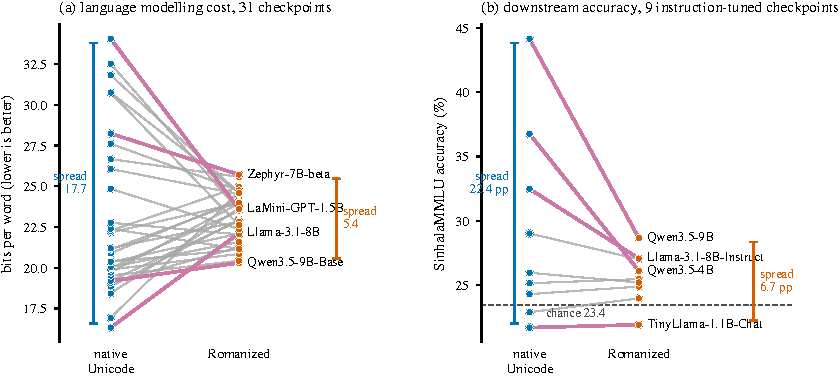
\includegraphics[width=\textwidth]{figures/fig1_flattening.pdf}
\caption{Romanization flattens the field. (a) Language modelling cost in bits per
word for 31 checkpoints. Word counts are identical within a pair, so the two
columns are directly comparable. Native-script cost varies by 17.7 bits across
checkpoints; Romanized cost varies by 5.4, and crossing lines mark the twelve
checkpoints that are cheaper on Romanized text. (b) SinhalaMMLU accuracy for the
instruction-tuned checkpoints. A 22.4 point spread becomes 6.7, and no checkpoint
finishes more than 5.3 points above chance. LaMini-GPT-1.5B is omitted from (b)
because it produces unparseable output on 95.9\% of native-script items; it
appears in Table~\ref{tab:main}.}
\label{fig:flat}
\end{figure*}

\begin{table*}[t]
\centering\small
\setlength{\tabcolsep}{2.5pt}
\begin{tabular}{@{}lr rrr c@{\hspace{4pt}}r rr rr r rr r@{}}
\toprule
& & \multicolumn{5}{c}{\textbf{SinhalaMMLU} (6{,}879 items)}
& \multicolumn{5}{c}{\textbf{SOLD} (2{,}500 items)}
& \multicolumn{2}{c}{\textbf{Invalid \%}} & \\
\cmidrule(lr){3-7}\cmidrule(lr){8-12}\cmidrule(lr){13-14}
& & \multicolumn{2}{c}{Acc.\ \%} & & &
& \multicolumn{2}{c}{macro-F1} & \multicolumn{2}{c}{\mcc} & & & & \\
\textbf{Checkpoint} & \textbf{B} & U & R & $\Delta$ & 95\% CI & $p_{\text{Holm}}$
& U & R & U & R & $p_{\text{Holm}}$ & U & R & $\tau$ \\
\midrule
\rows{tables/tab_extrinsic_main.tex}
\bottomrule
\end{tabular}
\caption{Downstream results, ordered by size. U is native Unicode, R is
Romanized, $\Delta$ is the paired difference in points and $p_{\text{Holm}}$ is
McNemar's test corrected across checkpoints within a task. $\mcc$ is Matthews
correlation and its $p_{\text{Holm}}$ comes from a paired bootstrap. $\tau$ is the
ratio of Romanized to native input tokens on SinhalaMMLU, below one for every
checkpoint. Invalid \% is the share of unparseable generations, on SinhalaMMLU.
$\dagger$ marks checkpoints passing the competence screen of \S\ref{sec:screen}.
Global PIQA is in Appendix Table~\ref{tab:piqa}.}
\label{tab:main}
\end{table*}

\subsection{You can only lose what you have}
\label{sec:law}

The relationship in the previous paragraph is remarkably tight. Writing headroom
as native accuracy minus chance, a linear fit across the nine parseable
checkpoints gives
\begin{equation}
\text{loss} = 0.78 \times \text{headroom} - 0.87,
\label{eq:law}
\end{equation}
with $R^2 = 0.97$ and $p = 1.9 \times 10^{-6}$ (Figure~\ref{fig:floor}a).
Romanization removes roughly four fifths of whatever native-script ability a
checkpoint had.

A single regression on nine points is thin evidence, so we test the same relation
inside the benchmark, where the units are items rather than models. Splitting
SinhalaMMLU into its 16 non-empty domain by difficulty cells and computing
headroom and loss per cell for the competent cohort gives a slope of 0.58 with
$R^2 = 0.83$ and $p = 9.8 \times 10^{-7}$ (Spearman $0.85$). The two
decompositions are independent, one across models and one across content, and
they agree.

Table~\ref{tab:strata} shows the strata. Loss falls monotonically with difficulty,
8.6 points on Easy items, 7.2 on Medium and 5.2 on Hard, and the interaction with
difficulty is significant in the item-clustered logistic fit ($p = 0.007$). Hard
items lose less because models are nearer chance on them in both conditions. By
domain, Social Science loses most at 11.8 points and is also where native-script
accuracy is highest, while Humanities, the largest domain at 3{,}341 items, loses
4.8 and has lower native accuracy. The pattern is uncomfortable for benchmark
design: the harder and less well-served a slice of a benchmark is, the smaller the
script effect it can reveal.

\begin{table}[t]
\centering\small
\setlength{\tabcolsep}{4pt}
\begin{tabular}{@{}lrrrrr@{}}
\toprule
\textbf{Stratum} & \textbf{Items} & \textbf{U \%} & \textbf{R \%}
& \boldmath$\Delta$ & \boldmath$p_{\text{Holm}}$ \\
\midrule
\rows{tables/tab_strata.tex}
\bottomrule
\end{tabular}
\caption{SinhalaMMLU by stratum, pooled over the five competent checkpoints. Item
counts are per checkpoint. Domains are ordered by loss.}
\label{tab:strata}
\end{table}

\subsection{Offensive-language detection: accuracy hides the damage}

SOLD is where the choice of metric decides the conclusion. Accuracy falls by only 1.6
to 11.3 points against a 59.4\% majority baseline, so three checkpoints look almost
unaffected. Matthews correlation says otherwise (Figure~\ref{fig:floor}b).
Qwen3.5-9B goes from 0.280 to 0.069, keeping 24\% of its signal,
Qwen2-7B-Instruct from 0.148 to 0.042, keeping 29\%, and Llama-3.1-8B-Instruct from
0.259 to 0.105, keeping 40\%. Four of the five checkpoints with a real native-script
signal lose significantly under Holm correction and the median keeps 40\%. The
mechanism is a retreat toward trivial behaviour: Qwen2-7B-Instruct more than doubles
its rate of predicting the offensive class, 10.5\% to 23.4\%, without becoming more
accurate, and Hormoz-8B does the same from 9.8\% to 20.7\%. A deployment tracking
accuracy here would see a 5 point wobble while over half the usable signal
disappeared.

\begin{figure}[t]
\centering
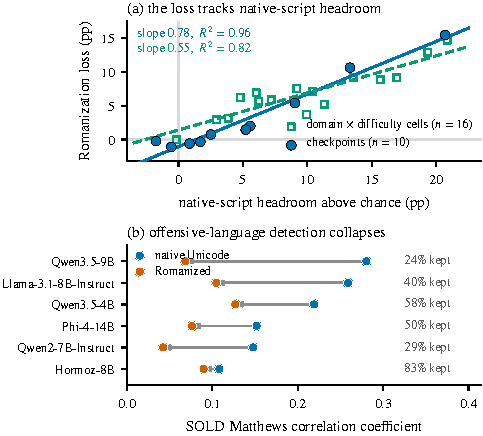
\includegraphics[width=\columnwidth]{figures/fig3_floor_effect.pdf}
\caption{(a) Romanization loss against native-script headroom above chance, across
checkpoints and independently across the 16 domain by difficulty cells of
SinhalaMMLU. (b) Matthews correlation on SOLD for the five checkpoints with a
real native-script signal, with the percentage retained under Romanization.}
\label{fig:floor}
\end{figure}

\subsection{Global PIQA is underpowered, and says so}

No checkpoint is above chance on the native-script condition of Global PIQA, so the
screen admits none, and with 100 items and a median of 36 discordant pairs no
comparison is significant. The direction is consistent, seven of nine parseable
checkpoints dropping, but a sign test gives $p = 0.18$ and pooling the cohort gives a
4.6 point gap at $p = 0.10$. We report this as a null result rather than
corroboration. A 100-item set cannot resolve effects of the size we measure
elsewhere, which is worth saying plainly given how often small multilingual splits
are read as evidence.

\subsection{Two things it is not}
\label{sec:controls}

\paragraph{Not token fragmentation.} The natural explanation for a Romanized penalty
is that romanization shatters words into more tokens. For Sinhala the opposite holds.
The native script costs a median 9.5 tokens per word against 2.09 for its
romanization, because these tokenizers largely fall back to bytes on Sinhala. Every
one of the ten checkpoints receives \emph{fewer} tokens in the Romanized condition on
all three tasks, a median ratio of 0.48 on SinhalaMMLU (column $\tau$ of
Table~\ref{tab:main}). Models get shorter, more compactly encoded input and do worse.
Splitting items into terciles by how much romanization inflates tokens gives no
monotone pattern either, with losses of 5.9, 7.5 and 7.2 points. The gap reflects
what is missing from pretraining, not how the input is chopped up. BLOOM illustrates
this: its pretraining corpus covers 46 languages and Sinhala is not one of them
\citep{laurencon-etal-2023-roots, lescao-etal-2023-bloom}, and it sits at the bottom
on native Sinhala while being unremarkable on Romanized text.

\paragraph{Not output degeneration.} A model could score at chance by emitting one
constant answer. For the competent cohort the share of answers on the most frequent
option is 37.0\% natively and 38.6\% under romanization (Wilcoxon $p = 0.63$), and
among the five competent checkpoints the invalid rate never exceeds 0.03\% in
either condition. The models keep answering across the option set. They are simply
wrong.

% =============================================================================
\section{Do Intrinsic Metrics Predict Downstream Fragility?}
\label{sec:linkage}

Can a cheap intrinsic measurement stand in for an expensive downstream one?
Table~\ref{tab:linkage} answers this for the nine checkpoints measured both ways.
Absolute native-script bits per byte predicts the SinhalaMMLU gap
($\rho = -0.90$, $p = 0.0009$) and the loss of Matthews correlation on SOLD
($\rho = -0.82$, $p = 0.007$). Lower bits per byte means a larger script gap, which
is the floor effect of \S\ref{sec:law} seen from the intrinsic side.

The negative result is the more useful one. The bits-per-byte \emph{gap} between
conditions, the natural analogue of the degradation ratio prior work reports,
predicts nothing ($\rho = -0.07$, $p = 0.86$), and neither does the perplexity
ratio ($\rho = -0.53$, $p = 0.14$). The widely reported quantity is the wrong one to
act on. To anticipate how much a model will suffer on Romanized Sinhala, measure how
good it is at native Sinhala, tokenizer-independently.

\begin{table}[t]
\centering\small
\setlength{\tabcolsep}{4pt}
\begin{tabular}{@{}lrrrr@{}}
\toprule
& \multicolumn{2}{c}{\textbf{MMLU gap}} & \multicolumn{2}{c}{\textbf{SOLD} $\Delta\mcc$} \\
\cmidrule(lr){2-3}\cmidrule(lr){4-5}
\textbf{Intrinsic predictor} & $\rho$ & $p$ & $\rho$ & $p$ \\
\midrule
\rows{tables/tab_linkage.tex}
\bottomrule
\end{tabular}
\caption{Spearman correlations between intrinsic measurements and downstream
script effects, over the nine parseable checkpoints. Levels predict; gaps and
ratios do not.}
\label{tab:linkage}
\end{table}

% =============================================================================
\section{Discussion}
\label{sec:discussion}

Three things follow for practice. First, a benchmark reporting perplexity across
model families on a script that tokenizers handle unevenly is reporting tokenizer
behaviour, and for Sinhala this inverts both the model ranking and the conclusion
about scale. Bits per byte costs nothing extra on the same forward passes. Second,
script robustness cannot be read off a group average: six of our ten checkpoints sit
at chance and contribute a zero gap by construction, and the same trap operates inside
a benchmark, where the hardest strata reveal the smallest effects. Any robustness
claim needs a competence screen and a stated guessing baseline. Third, the models best at native Sinhala have the most to lose, so
picking by native-script scores and serving Romanized users selects for the largest
drop.

The flattening result also says where effort should go. Romanized ability is nearly
constant across 31 checkpoints spanning a 42-fold parameter range, and none beats a
character bigram fit on 400 sentences. That is missing data, not something scale will
fix: the remedies are transliteration before inference and Romanized pretraining
data.

% =============================================================================
\section*{Limitations}

\paragraph{One language.} Everything here is Sinhala. The mechanism we describe,
a floor effect that makes robustness gaps proportional to native ability, should
generalise to any language with a dominant Romanized register, but we have not
shown that. Hindi, Urdu, Nepali, Tamil and Arabic dialects are the obvious tests,
and \citet{khullar-etal-2025-scriptgap} report compatible magnitudes for the first
three.

\paragraph{The Romanized side of the downstream sets is synthetic.} We
transliterate native-script items rather than collecting human-typed Romanized
versions of them, because no such parallel resource exists at this scale. Our
transliterator is the best of four on 755{,}000 human references, and its residual
error is a spelling regularity that should make the text easier rather than harder,
but it is still not what a person would type. The intrinsic results do not share
this limitation, since their Romanized side was typed by native speakers, and they
show the same flattening. A human-written Romanized version of even a few hundred
SinhalaMMLU items would settle the question.

\paragraph{Open weights only, and small ones.} We evaluate open checkpoints up to
9B for the downstream tasks. Frontier proprietary models are much stronger on
Sinhala \citep{pramodya-etal-2025-sinhalammlu} and therefore have far more
headroom, so Equation~\ref{eq:law} predicts larger absolute losses for them. That
prediction is untested here.

\paragraph{Zero-shot only.} We use one template, zero-shot, greedy. This measures
what a user gets out of the box, not the ceiling. Few-shot prompting,
transliterate-then-infer, or Romanized fine-tuning could all narrow the gap, and
we do not measure by how much.

\paragraph{Two checkpoints cannot do the task.} LaMini-GPT-1.5B and
TinyLlama-1.1B-Chat produce unparseable output on most native-script items of at
least one task. Their apparent improvement under Romanization is an artifact of
that failure, not a script effect, which is why the competence screen exists.

\section*{Ethics Statement}

All datasets are public research releases used within their licences and for
evaluation only, which matters for Global PIQA, whose licence forbids training.
SOLD contains offensive social media text; it is already pseudonymised upstream,
with user mentions replaced by placeholders, and we neither collected nor
re-annotated any of it. We add no new human annotation and no new data collection.

The practical risk our results speak to is deployment. A moderation or support
system validated on native-script Sinhala and serving Romanized users will look
far better in evaluation than in the field, and on SOLD that failure is invisible
in accuracy while more than half the usable signal is gone. Publishing the size of
that gap, and a screen that stops averaging from hiding it, is the useful response.
Our transliterator collapses several Sinhala consonant distinctions, matching
casual Singlish practice, so it is a tool for building evaluation data and not for
rendering names or other text where those distinctions carry meaning.

\section*{Acknowledgments}

Omitted for anonymous review.

\bibliography{custom}

% =============================================================================
\appendix

\section{Prompt Template}
\label{sec:prompts}

One template is used for every dataset and both script conditions. Multiple
choice, with the option count $n$ and the domain name inserted where available:

\begin{quote}\small\ttfamily
This is a multiple-choice question related to the \{domain\}. Choose the correct
or most appropriate answer from answers 1/.../$n$ for the following question. Do
not repeat the question or text in your response. Respond with only the number
(1/.../$n$) and nothing else.\\
Question: \{question\}\\
1. \{option 1\} ... $n$. \{option $n$\}\\
Answer:
\end{quote}

Binary classification:

\begin{quote}\small\ttfamily
Classify the following Sinhala text as either 'NOT' (not offensive) or 'OFF'
(offensive). Do not repeat the question or text in your response. Respond with
only 'NOT' or 'OFF' and nothing else.\\
Text: \{text\}\\
Answer:
\end{quote}

Prompts are rendered through each checkpoint's own chat template. For checkpoints
that emit reasoning traces by default we disable that behaviour identically in
both script conditions. Decoding is greedy at temperature 0 with at most 40 new
tokens and inputs truncated at 4{,}096 tokens.

\section{Checkpoints}
\label{sec:models}

Table~\ref{tab:modelids} lists all 31 checkpoints with their Hugging Face
identifiers and their tokenizer fertility on the parallel corpus. Note the
consistency of Romanized fertility, between 1.9 and 2.4 tokens per word, against
a range of 4.3 to 14.2 on the native script.

\begin{table*}[t]
\centering\small
\setlength{\tabcolsep}{5pt}
\begin{tabular}{@{}lrlrr@{}}
\toprule
& & & \multicolumn{2}{c}{\textbf{tokens / word}} \\
\cmidrule(lr){4-5}
\textbf{Checkpoint} & \textbf{B params} & \textbf{Hugging Face identifier} & Unicode & Romanized \\
\midrule
\rows{tables/tab_model_ids.tex}
\bottomrule
\end{tabular}
\caption{All evaluated checkpoints, with Hugging Face identifiers and tokenizer
fertility on the parallel corpus. $\ddagger$ marks the ten used for the downstream
evaluation. Native-script fertility varies by more than a factor of three across
tokenizers, whereas Romanized fertility is nearly constant.}
\label{tab:modelids}
\end{table*}

\section{Global PIQA and the $n$-gram Reference}
\label{sec:piqa}

Table~\ref{tab:piqa} gives the per-checkpoint Global PIQA results omitted from
Table~\ref{tab:main}, and Figure~\ref{fig:ngram} plots the $n$-gram comparison of
Table~\ref{tab:ngram}.

\begin{table}[t]
\centering\footnotesize
\setlength{\tabcolsep}{2.2pt}
\begin{tabular}{@{}lrrrcrrr@{}}
\toprule
& \multicolumn{2}{c}{Acc.\ \%} & & \textbf{disc.} & & \multicolumn{2}{c}{\textbf{Inv.\ \%}} \\
\cmidrule(lr){2-3}\cmidrule(lr){5-5}\cmidrule(lr){7-8}
\textbf{Checkpoint} & U & R & \boldmath$\Delta$ & \textbf{b/c}
& \boldmath$p_{\text{Holm}}$ & U & R \\
\midrule
\rows{tables/tab_piqa.tex}
\bottomrule
\end{tabular}
\caption{Global PIQA, 100 items. ``disc.\ b/c'' are the discordant pair counts
entering McNemar's test. No checkpoint is above chance in the native-script
condition and no comparison survives correction, so we treat this task as
underpowered rather than as corroboration.}
\label{tab:piqa}
\end{table}

\begin{figure}[t]
\centering
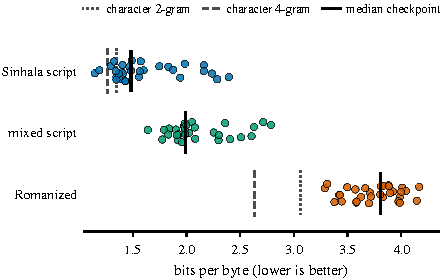
\includegraphics[width=\columnwidth]{figures/fig4_ngram_reference.pdf}
\caption{Bits per byte for all 31 checkpoints in each script condition, with
held-out character $n$-gram references. The mixed-script corpus is not parallel,
so no reference is shown for it.}
\label{fig:ngram}
\end{figure}

\section{Full Intrinsic Results}
\label{sec:fullintrinsic}

Table~\ref{tab:intrinsicfull} gives every metric for every checkpoint in all three
script conditions, corpus-pooled as in Equation~\ref{eq:bpb}.

\begin{table*}[t]
\centering\scriptsize
\setlength{\tabcolsep}{3pt}
\begin{tabular}{@{}lr rrr rrr rrr@{}}
\toprule
& & \multicolumn{3}{c}{\textbf{Native Unicode}} & \multicolumn{3}{c}{\textbf{Romanized}}
& \multicolumn{3}{c}{\textbf{Mixed script}} \\
\cmidrule(lr){3-5}\cmidrule(lr){6-8}\cmidrule(lr){9-11}
\textbf{Checkpoint} & \textbf{B} & PPL & \bpb{} & \bpw{}
& PPL & \bpb{} & \bpw{} & PPL & \bpb{} & \bpw{} \\
\midrule
\rows{tables/tab_intrinsic_full.tex}
\bottomrule
\end{tabular}
\caption{Corpus-pooled intrinsic metrics for all 31 checkpoints, sorted by
native-script bits per byte. $\ddagger$ marks the checkpoints also evaluated
downstream. Bits per character are omitted because they are a fixed multiple of
bits per byte within a script, $2.651\times$ for native Sinhala and $1.003\times$
for its romanization. Note that the PPL and \bpb{} orderings disagree almost
completely.}
\label{tab:intrinsicfull}
\end{table*}

\section{Reproducibility}
\label{sec:repro}

Every number in this paper is produced by scripts that read only the per-item
model outputs, so the tables and figures cannot drift from the data. We release
the frozen evaluation sets with both script conditions paired per record, all
per-item generations for every checkpoint, the analysis and figure scripts, and
the transliterator: \anonrepo. The transliterator is also available as
\texttt{pip install \pkg}, documented at \pkgurl.

Intrinsic evaluation scores 46{,}500 sequences (31 checkpoints, 1{,}500 sequences
each). Downstream evaluation produces 189{,}580 generations (10 checkpoints,
9{,}479 items, two script conditions). Both use fp16 on commodity dual-T4 GPUs.
Greedy decoding and a fixed template make the downstream runs deterministic up to
GPU non-determinism, and the transliteration and data preparation steps are fully
deterministic with byte-identical outputs recorded as SHA-256 digests.

\end{document}
